\section{Evaluation}
\label{sub:sl-evaluation}
SchemaLine was integrated into an existing visual analytics system to evaluate its usefulness in making sense of temporal relationships in intelligence analysis. The integration will be discussed next and followed by a sensemaking case study.

\subsection{Application}
% Overview of INVISQUE
We integrate SchemaLine into INVISQUE~\cite{Wong2011} -- a visual analytics system designed for interactive exploration of text documents. INVISQUE provides full-text search and organizes the search results into a two-dimensional canvas, with each dimension representing a configurable attribute. For example, it may be useful to order academic articles horizontally by publication date and vertically by citation count. Search results are shown as a cluster of \emph{index-cards}, each representing a document with selected information such as publication title, date, keywords and authors. \autoref{fig:invisque} shows a screenshot of INVISQUE.

\begin{figure}
	\centering
	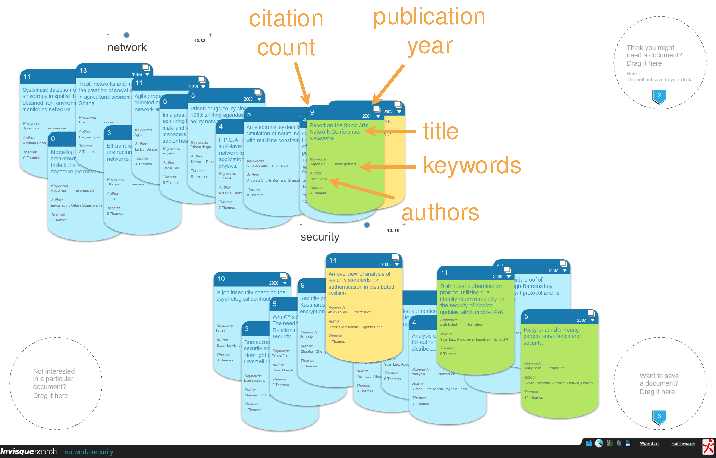
\includegraphics[width=\linewidth]{invisque}
	\caption[INVISQUE interface]{INVISQUE interface. It shows two clusters of search results for ``network'' and ``security'' from a publication dataset. Each index-card in a cluster represents an article with meta information displayed on it. \is{Wong2011}}
	\label{fig:invisque}
\end{figure}

% Integration
We add an \emph{annotation} feature to allow analysts to record their thoughts while reading documents. Technically, the association between an annotation and its containing document should be saved for potential provenance retrieval. These annotations are important to analysts, thus are also displayed on the index-cards together with other meta information. The annotations are used  as the input \emph{events} of the SchemaLine visualization. SchemaLine is placed at the bottom of INVISQUE (\autoref{fig:invisque-schemaline}). After the analyst makes a note, or annotation, it is immediately added to SchemaLine as a new event. Double clicking on an event will open the document containing that note as an index-card, enabling the analyst to quickly reexamine the original information source.

\begin{figure}
	\centering
	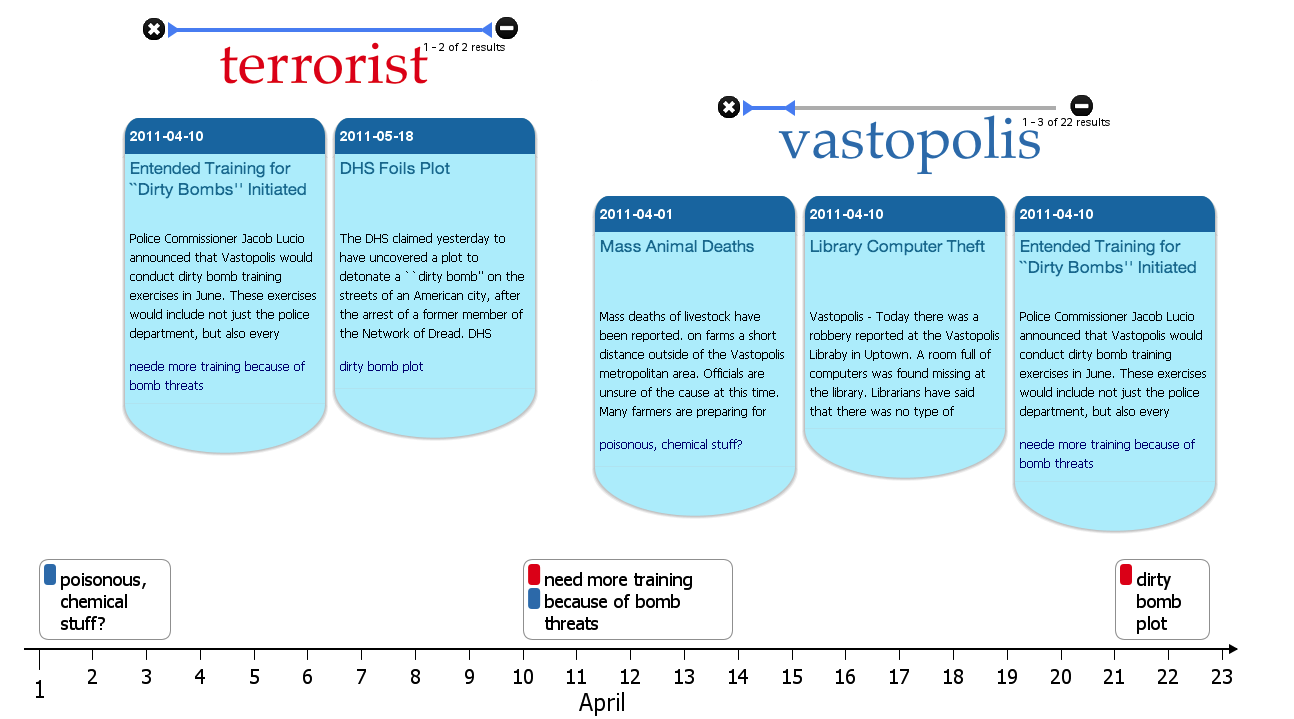
\includegraphics[width=\linewidth]{invisque-schemaline}
	\caption[INVISQUE with SchemaLine at the bottom]{INVISQUE with SchemaLine at the bottom. The timeline consists of three events, which are notes taken by an analyst. Color coded categories of events indicate keywords that were searched for.}
	\label{fig:invisque-schemaline}
\end{figure}

% Attribute mapping
The \emph{temporal information} of documents, such as ``publication date'', is initially assigned to that of events, and can be corrected later by analysts. This feature can be useful because the report date is not necessary the same as the date when the event actually occurred. For example, a news article published today can be written about a bomb attack that happened several days ago. The analyst can make the correction by dragging an event with the right mouse button along the time axis and dropping it at the desired date.

The \emph{label} of an event simply maps to the content of an annotation itself. In INVISQUE, we color code search keywords that contain annotated documents, and use them as \emph{categories} for events. Because a document can be returned from different searches, it can thus contain multiple categories. This mapping provides context for the annotations: what did I search for (the original keyword) and what are other related concepts (other search keywords returning the same document)? This context may help analysts discover interesting patterns through their annotations. \autoref{fig:invisque-schemaline} shows a screenshot of INVISQUE with SchemaLine integrated.

\subsection{Case Study}

\subsubsection{Design}

\paragraph{Method}
Evaluating the usefulness of SchemaLine in supporting sensemaking can be categorized as \emph{evaluating visual data analysis and reasoning} -- one of the seven scenarios in evaluating information visualization proposed by Lam~et~al.~\cite{Lam2012}. The goal of this evaluation scenario is to explore whether and how a visualization tool supports participants to make sense of the given tasks and generate relevant knowledge. During solving sensemaking tasks, participants may employ various strategies. Their processes and outcomes are also highly context-sensitive, making it difficult to quantify and compare their performance. Therefore, sensemaking evaluations are typically case studies with real-world tasks performed by domain experts. We conducted a case study to explore how SchemaLine supports analysts to solve an intelligence analysis task, focusing on how it enables them to perform sensemaking activities in the Data--Frame model. However, due to a limited access to these resources, we instead use a realistic investigative task with graduate students.

\paragraph{Task}
We used the task from Mini Challenge 3 of the IEEE VAST Challenge 2011~\footnote{\url{http://hcil2.cs.umd.edu/newvarepository/VAST Challenge 2011/challenges/MC3 - Investigation into Terrorist Activity/}}, which requires the participants to identify any imminent threats from the given dataset. We chose this task because it resembles a real intelligence task, demanding analysts to read many documents, extract relevant pieces of evidence and assemble them in order to derive insight and find a reasonable answer to the given question. Also, the solution was provided and well-tested by the community, making it possible to assess participants' performance. The participants were given INVISQUE with SchemaLine integrated to solve the task.

\paragraph{Dataset}
The original dataset contains more than four thousand news reports, 36 of which are relevant to criminal activities and are manually added by the Challenge committee. Both participants in our pilot test failed to find any imminent threats after one and a half hours. Most of their time was spent on reading long (more than 500 words) but irrelevant documents. The reason could be that INVISQUE does not support text-mining features such as entity extraction, which is crucial in analyzing a large document collection. However, the goal of this evaluation was to assess how SchemaLine can provide additional sensemaking support to INVISQUE rather than assessing INVISQUE itself. Therefore, in the main study, we removed all irrelevant documents that are not part of the ground truth to make the dataset size more manageable. The new dataset only contains the 36 relevant documents, 29 of which are correct answers including five criminal activities: food poisoning (13 documents), hacking (3), dirty bomb (6), arms trafficking (4), and money laundering (3). Other documents are isolated cases, acted as false leads. We expected that participants could complete the task within a reasonable amount of time, without affecting the goal of the study.

\paragraph{Participants and Procedure}
We were unable to recruit real intelligence analysts for the study. Instead, we recruited three graduate students with different backgrounds:  one in visual analytics (surrogate for visualization expert -- \textbf{P1}), one in law (surrogate for domain expert -- \textbf{P2}), and one in computer network (neutral background -- \textbf{P3}). After being introduced features of INVISQUE and SchemaLine, participants had a chance to practice with a trial sensemaking task for 15 minutes. The main task was followed and lasted for one hour. The participants were asked to report the criminal activities they had discovered with supporting evidence. Semi-structured interviews were followed to gain deeper understanding of the sensemaking processes.

\subsubsection{Results and Discussion}
We first summarize the three sessions and present our collective findings next.

\paragraph{Participant 1}
\textbf{P1} began searching for ``bomb'', examined the search results, and searched for  a refined keyword ``dirty bomb''. He took notes in three documents and then linked these notes together (\emph{connect data and a frame}). He then searched for ``Network of Dread'', which was mentioned in one of documents related to the dirty bomb attack. He took a note in the new returned document and dropped it onto the ``dirty bomb'' schema (\emph{elaborate the frame}). While investigating, he encountered an article about a man carrying a frozen turkey having wires coming out of it, which was suspected as a bomb. At first, he dropped the ``turkey bomb'' note onto the ``dirty bomb'' schema. Then, he wondered whether it was a real bomb. After thinking for a while, he removed it out of the schema (\emph{preserve the frame}). \textbf{P1} found the ``dirty bomb'' attack with 4/6 correct pieces of evidence. \textbf{P1} took many notes in documents related to the ``food poisoning'' case; however, he could not link them together because he said that ``I'm not familiar with bio-attack so I couldn't think of it as a threat''.

\paragraph{Participant 2}
\textbf{P2} took an overview step before searching. He quickly looked at all 36 document titles to have a glimpse of the dataset as well as to detect potential search keywords. Then he searched for ``animal deaths'', read the results, took notes and grouped them together (\emph{connect data and a frame}). He was satisfied with the evidence he found for that crime and switched to read another interesting article ``Library Computer Left'' he came across. From that, he searched for several related terms such as ``computer'' and ``hackers''. He figured out that a group called ``F-alliance'' stole computers from the library and attempted to hack a bank. He dropped a ``computer stolen'' note on top of a ``bank hacking'' note to form a new explanation for the case (\emph{connect data and a frame}). He found another article related to hacking but he said ``I won't drop it to this group because it's just an announcement from the government about potential threats'' (\emph{preserve the frame}). During further investigation, he created another group of notes related to ``bioterrorism'' and ``Prof. Patino''. Then, when figuring out that the reason of the mass deaths is a spore-forming microbe, which is also mentioned in Prof. Patino's talk, he dropped that new group onto the ``animal deaths'' group to combine all notes together because he thought that they were related (\emph{merge frames}). Observing the order of events in the new group on the timeline, he said ``The equipment of Patino was stolen after the animal deaths report, so they couldn't be used in that case. This is the group of a potential threat in using bioterrorism.'' (\emph{elaborate the frame}). \textbf{P2} found the ``hacking'' case with 2/3 correct pieces of evidence and the ``food poisoning'' case with 9/13 correct pieces of evidence. \autoref{fig:evaluation} shows the computer screen of \textbf{P2} when he reported his findings.

\begin{figure}
	\centering
	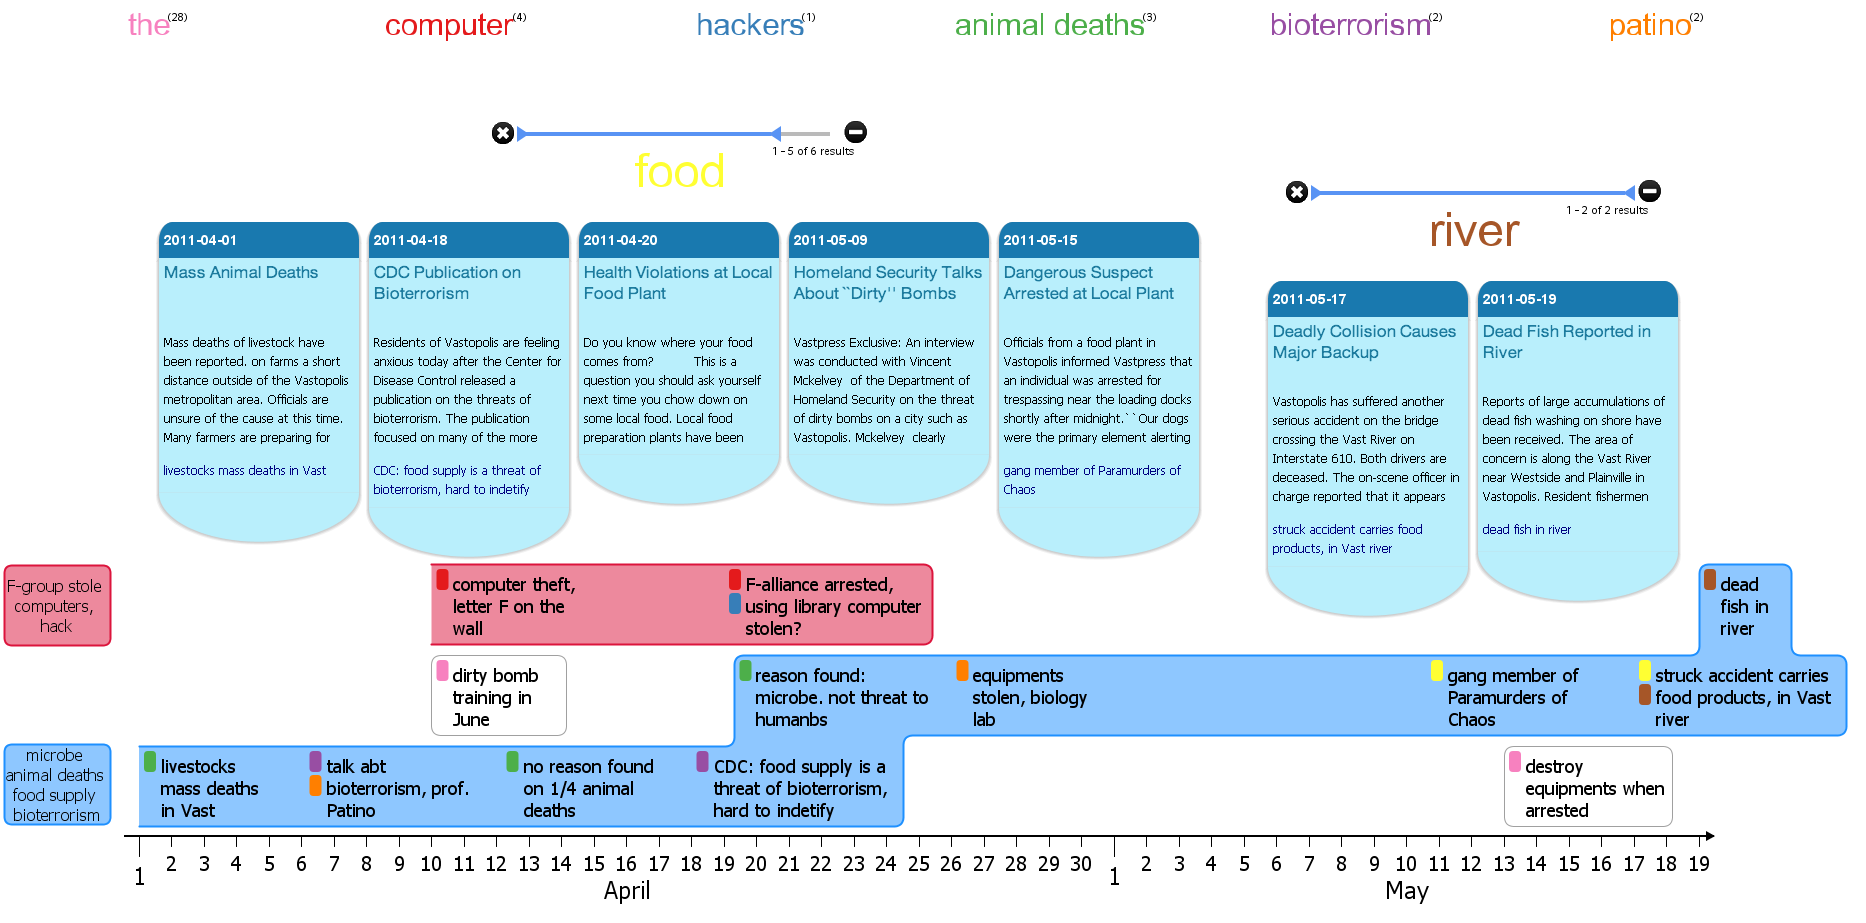
\includegraphics[width=\linewidth]{evaluation}
	\caption[Final screen of participant \textbf{P2}]{Final screen of participant \textbf{P2}. Top: a trail of his keyword searches, collapsed after being read. Middle: search results in index-card metaphor. Bottom: two schemas containing notes as supporting evidence of criminal activities he found.}
	\label{fig:evaluation}
\end{figure*}

\paragraph{Participant 3}
\textbf{P3} searched for a few keywords related to criminal activities before examining the search results such as ``bomb'', ``terrorism'', ``money'' and ``hack''. He took and group notes about ``money laundering'' together (\emph{connect data and a frame}). Then, he read articles from ``terrorism'' search results. He followed the article content to search for relevant information such as ``Paramurderers of Chaos'' -- a terrorist group. During further investigation, similar to \textbf{P2}, he also combined two groups of notes -- ``Paramurderers of Chaos'' and ``food supply'' -- together when discovering evidence linking the two groups (\emph{merge frames}). When presenting his findings, he shared that SchemaLine prompted him to look for missing information. ``I noticed the gap between these two events [pointing to the timeline]; then I knew I probably missed something there'' (\emph{question the frame}). \textbf{P3} found the ``food poisoning'' case with 6/13 correct pieces of evidence, and a perfect 3/3 pieces of evidence in the ``money laundering'' case.

\paragraph{Discussion}
The evaluation revealed some useful insights in the use of SchemaLine for supporting sensemaking in intelligence analysis.

\subparagraph{Effective Externalization of Sensemaking}
Three participants applied different sensemaking strategies. \textbf{P1} started with a potential search keyword for criminal activities and kept following the search results. \textbf{P2} initially scanned the titles of all documents to have an overview of the dataset. \textbf{P3} planned ahead what he wanted to search for and sequentially executed it. However, all of them extensively took notes and constructed explanatory frames from them. These frames presented various forms: a concept (bioterrorism), a criminal activity (dirty bomb), a person (Prof. Patino) and a group of people (Paramurderers of Chaos). All participants also employed a variety of sensemaking activities described in the Data--Frame model, supported through fluid interaction in SchemaLine: connect data and a frame, elaborate the frame, question the frame preserve the frame and merge frames.

\subparagraph{Temporal Schematization}
All participants appreciated the automatic addition of analyst notes from INVISQUE to SchemaLine. \textbf{P1} thought that he would have a problem if the system did not support that: ``I can remember what happened but it was difficult to remember when they happened''. They found that the chronological order of events provides cues to them to construct the story lines. \textbf{P2} shared that he read the news about the robbery at Vastopolis university and the Prof. Patino's talk about bioterrorism. However, he did not have any insight at that time. When looking at his two notes on the timeline, he thought that the extremely expensive equipment in Prof. Patino's lab could be the reason for the robbery.

\subparagraph{Intuitive Interface}
All participants commented that the interaction between data and frame was very intuitive. \textbf{P1} said ``I think I don't even need training and still can figure out how it works''. \textbf{P3} appreciated the transition effect when adding or removing notes because ``it helped me to understand what is going on''. All participants were confident while presenting their analyses. \textbf{P3} even opened the original document (double-clicking on the note) several times to highlight the relevant text. He said that the connection between the note and the containing document enabled him to quickly find the information source when needed.